%  LaTeX support: latex@mdpi.com
%  For support, please attach all files needed for compiling as well as the log file, and specify your operating system, LaTeX version, and LaTeX editor.

%=================================================================
% pandoc conditionals added to preserve backwards compatibility with previous versions of rticles

\documentclass[nutrients,article,submit,moreauthors,pdftex]{Definitions/mdpi}


%% Some pieces required from the pandoc template
\setlist[itemize]{leftmargin=*,labelsep=5.8mm}
\setlist[enumerate]{leftmargin=*,labelsep=4.9mm}


%--------------------
% Class Options:
%--------------------

%---------
% article
%---------
% The default type of manuscript is "article", but can be replaced by:
% abstract, addendum, article, book, bookreview, briefreport, casereport, comment, commentary, communication, conferenceproceedings, correction, conferencereport, entry, expressionofconcern, extendedabstract, datadescriptor, editorial, essay, erratum, hypothesis, interestingimage, obituary, opinion, projectreport, reply, retraction, review, perspective, protocol, shortnote, studyprotocol, systematicreview, supfile, technicalnote, viewpoint, guidelines, registeredreport, tutorial
% supfile = supplementary materials

%----------
% submit
%----------
% The class option "submit" will be changed to "accept" by the Editorial Office when the paper is accepted. This will only make changes to the frontpage (e.g., the logo of the journal will get visible), the headings, and the copyright information. Also, line numbering will be removed. Journal info and pagination for accepted papers will also be assigned by the Editorial Office.

%------------------
% moreauthors
%------------------
% If there is only one author the class option oneauthor should be used. Otherwise use the class option moreauthors.

%---------
% pdftex
%---------
% The option pdftex is for use with pdfLaTeX. Remove "pdftex" for (1) compiling with LaTeX & dvi2pdf (if eps figures are used) or for (2) compiling with XeLaTeX.

%=================================================================
% MDPI internal commands - do not modify
\firstpage{1}
\makeatletter
\setcounter{page}{\@firstpage}
\makeatother
\pubvolume{1}
\issuenum{1}
\articlenumber{0}
\pubyear{2024}
\copyrightyear{2024}
%\externaleditor{Academic Editor: Firstname Lastname}
\datereceived{ }
\daterevised{ } % Comment out if no revised date
\dateaccepted{ }
\datepublished{ }
%\datecorrected{} % For corrected papers: "Corrected: XXX" date in the original paper.
%\dateretracted{} % For corrected papers: "Retracted: XXX" date in the original paper.
\hreflink{https://doi.org/} % If needed use \linebreak
%\doinum{}
%\pdfoutput=1 % Uncommented for upload to arXiv.org

%=================================================================
% Add packages and commands here. The following packages are loaded in our class file: fontenc, inputenc, calc, indentfirst, fancyhdr, graphicx, epstopdf, lastpage, ifthen, float, amsmath, amssymb, lineno, setspace, enumitem, mathpazo, booktabs, titlesec, etoolbox, tabto, xcolor, colortbl, soul, multirow, microtype, tikz, totcount, changepage, attrib, upgreek, array, tabularx, pbox, ragged2e, tocloft, marginnote, marginfix, enotez, amsthm, natbib, hyperref, cleveref, scrextend, url, geometry, newfloat, caption, draftwatermark, seqsplit
% cleveref: load \crefname definitions after \begin{document}

%=================================================================
% Please use the following mathematics environments: Theorem, Lemma, Corollary, Proposition, Characterization, Property, Problem, Example, ExamplesandDefinitions, Hypothesis, Remark, Definition, Notation, Assumption
%% For proofs, please use the proof environment (the amsthm package is loaded by the MDPI class).

%=================================================================
% Full title of the paper (Capitalized)
\Title{Substitution of red meat with legumes and risk of primary liver cancer in UK Biobank participants: a prospective cohort study}

% MDPI internal command: Title for citation in the left column
\TitleCitation{Substitution of red meat with legumes and risk of primary liver cancer in UK Biobank participants: a prospective cohort study}

% Author Orchid ID: enter ID or remove command
%\newcommand{\orcidauthorA}{0000-0000-0000-000X} % Add \orcidA{} behind the author's name
%\newcommand{\orcidauthorB}{0000-0000-0000-000X} % Add \orcidB{} behind the author's name


% Authors, for the paper (add full first names)
\Author{Niels Bock$^{1}$\href{https://orcid.org/0009-0005-7373-1589}
{\orcidicon}, Fie Langmann$^{1}$\href{https://orcid.org/0000-0003-3474-9346}
{\orcidicon}, Luke W. Johnston$^{1, 2}$\href{https://orcid.org/0000-0003-4169-2616}
{\orcidicon}, Daniel B. Ibsen$^{1, 2, 3, 4}$\href{https://orcid.org/0000-0002-7038-4770}
{\orcidicon}, Christina C. Dahm$^{1, *}$\href{https://orcid.org/0000-0003-0481-2893}
{\orcidicon}}


%\longauthorlist{yes}


% MDPI internal command: Authors, for metadata in PDF
\AuthorNames{Niels Bock, Fie Langmann, Luke W. Johnston, Daniel B. Ibsen, Christina C. Dahm}

% MDPI internal command: Authors, for citation in the left column
%\AuthorCitation{Lastname, F.; Lastname, F.; Lastname, F.}
% If this is a Chicago style journal: Lastname, Firstname, Firstname Lastname, and Firstname Lastname.
\AuthorCitation{Bock, N; Langmann, F; Johnston, LW; Ibsen, DB; Dahm, CC}

% Affiliations / Addresses (Add [1] after \address if there is only one affiliation.)
\address{%
$^{1}$ \quad Department of Public Health,
Aarhus University,
Aarhus, Denmark; \\
$^{2}$ \quad Steno Diabetes Center Aarhus,
Aarhus University Hospital,
Aarhus N, Denmark; \\
$^{3}$ \quad Department of Nutrition, Exercise and Sports,
University of Copenhagen,
Copenhagen, Denmark; \\
$^{4}$ \quad MRC Epidemiology Unit, School of Clinical Medicine,
University of Cambridge,
Cambridge, United Kingdom; \\
}

% Contact information of the corresponding author
\corres{Correspondence: \href{mailto:CCD@ph.au.dk}{\nolinkurl{CCD@ph.au.dk}}.}

% Current address and/or shared authorship








% The commands \thirdnote{} till \eighthnote{} are available for further notes

% Simple summary

%\conference{} % An extended version of a conference paper

% Abstract (Do not insert blank lines, i.e. \\)
\abstract{Purpose: Primary liver cancer is on the rise worldwide, partially due to poor diets and sedentary lifestyles. Shifting to more plant-based diets may lower the risk. We aimed to estimate the effect of replacing unprocessed red meat, processed red meat and total red meat with legumes on primary liver cancer in a free-living population. Methods: We analyzed data from 126,744 UK Biobank participants who completed \(\geq\) 2 24-hour diet recalls. Baseline characteristics were collected from the initial assessment visit. Information on liver cancer diagnoses was collected via external linkage to inpatient hospital episodes or central cancer registries. Cox proportional hazards regression models were used to estimate substitution of 15 g/day of legumes with 15 g/day of total red meat, unprocessed red meat or processed red meat on liver cancer risk, using the leave-one-out food substitution model. Results: During a median follow-up time of 11.3 years, 173 participants developed liver cancer. In the fully adjusted models, no association was observed when substituting 15 g/day of legumes with total red meat (HR: 1.02 (95\% CI 0.96-1.08)), unprocessed red meat (HR: 1.00 (95\% CI 0.94-1.06)) or processed red meat (HR: 1.09 (95\% CI 0.99-1.21)). Conclusion: Overall, little evidence of an association between replacing red meat with legumes and liver cancer was observed. Further research in larger study populations with longer follow-up time is warranted.}


% Keywords
\keyword{Food Substitutions; liver cancer; red meat; legumes.}

% The fields PACS, MSC, and JEL may be left empty or commented out if not applicable
%\PACS{J0101}
%\MSC{}
%\JEL{}

%%%%%%%%%%%%%%%%%%%%%%%%%%%%%%%%%%%%%%%%%%
% Only for the journal Diversity
%\LSID{\url{http://}}

%%%%%%%%%%%%%%%%%%%%%%%%%%%%%%%%%%%%%%%%%%
% Only for the journal Applied Sciences

%%%%%%%%%%%%%%%%%%%%%%%%%%%%%%%%%%%%%%%%%%

%%%%%%%%%%%%%%%%%%%%%%%%%%%%%%%%%%%%%%%%%%
% Only for the journal Data



%%%%%%%%%%%%%%%%%%%%%%%%%%%%%%%%%%%%%%%%%%
% Only for the journal Toxins


%%%%%%%%%%%%%%%%%%%%%%%%%%%%%%%%%%%%%%%%%%
% Only for the journal Encyclopedia


%%%%%%%%%%%%%%%%%%%%%%%%%%%%%%%%%%%%%%%%%%
% Only for the journal Advances in Respiratory Medicine
%\addhighlights{yes}
%\renewcommand{\addhighlights}{%

%\noindent This is an obligatory section in “Advances in Respiratory Medicine”, whose goal is to increase the discoverability and readability of the article via search engines and other scholars. Highlights should not be a copy of the abstract, but a simple text allowing the reader to quickly and simplified find out what the article is about and what can be cited from it. Each of these parts should be devoted up to 2~bullet points.\vspace{3pt}\\
%\textbf{What are the main findings?}
% \begin{itemize}[labelsep=2.5mm,topsep=-3pt]
% \item First bullet.
% \item Second bullet.
% \end{itemize}\vspace{3pt}
%\textbf{What is the implication of the main finding?}
% \begin{itemize}[labelsep=2.5mm,topsep=-3pt]
% \item First bullet.
% \item Second bullet.
% \end{itemize}
%}


%%%%%%%%%%%%%%%%%%%%%%%%%%%%%%%%%%%%%%%%%%


% tightlist command for lists without linebreak
\providecommand{\tightlist}{%
  \setlength{\itemsep}{0pt}\setlength{\parskip}{0pt}}

% From pandoc table feature
\usepackage{longtable,booktabs,array}
\usepackage{calc} % for calculating minipage widths
% Correct order of tables after \paragraph or \subparagraph
\usepackage{etoolbox}
\makeatletter
\patchcmd\longtable{\par}{\if@noskipsec\mbox{}\fi\par}{}{}
\makeatother
% Allow footnotes in longtable head/foot
\IfFileExists{footnotehyper.sty}{\usepackage{footnotehyper}}{\usepackage{footnote}}
\makesavenoteenv{longtable}


\usepackage{caption}
\captionsetup{font=small,justification=raggedright,singlelinecheck=false}
\captionsetup[table]{labelformat=default, labelsep=period, name=Table S}
\captionsetup[figure]{labelformat=default, labelsep=period, name=Figure S}
\usepackage{longtable, fancyhdr}
\usepackage{booktabs}
\usepackage{caption}
\usepackage{longtable}
\usepackage{rotating}
\usepackage{colortbl}
\usepackage{array}
\usepackage{anyfontsize}

\begin{document}



%%%%%%%%%%%%%%%%%%%%%%%%%%%%%%%%%%%%%%%%%%

\clearpage

\hypertarget{sec1}{%
\section{Supplementary materials}\label{sec1}}

\begin{figure*}[h]

{\centering 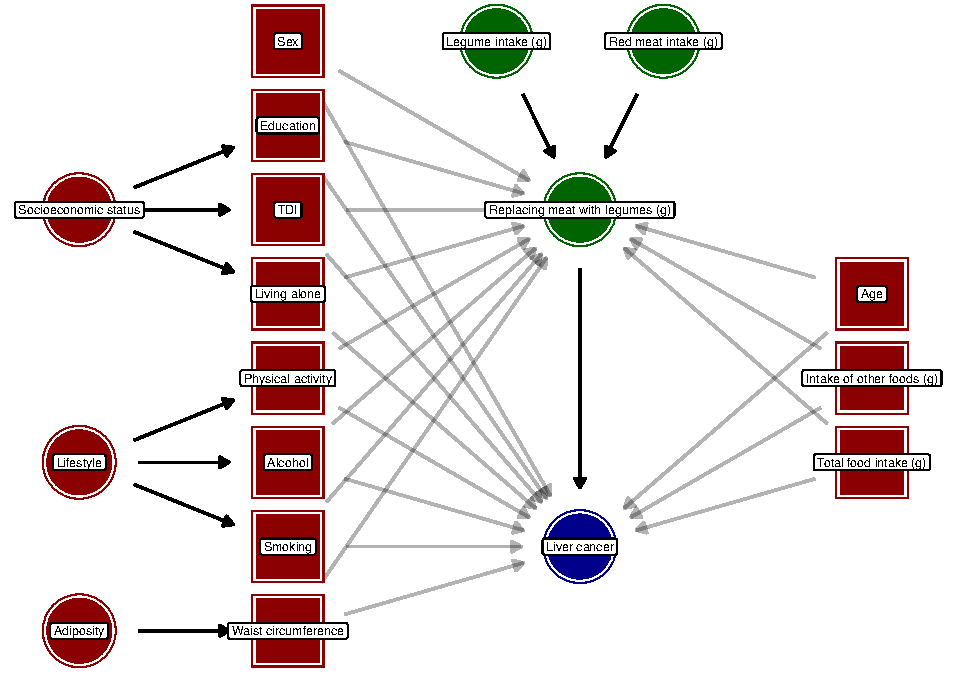
\includegraphics[width=1\linewidth,]{appendix-test_files/figure-latex/fig2-1}

}

\caption{Simplified directed acyclic graph (DAG) visualizing the hypothesised causal relationship between replacing red meat with legumes and liver cancer based on assumptions of biasing paths. Red nodes represent confounders. Square nodes represent the minimal sufficient adjustment set for estimating the effect of replacing red meat with legumes on liver cancer. Shadowed arrows represent biasing paths. DAG terminology demands visualisation of all hypothesized correlating relationships between variables, typically resulting in complex and hard-to-follow illustrations. To improve readability, inter-covariate arrows are hidden in the above DAG.}\label{fig:fig2}
\end{figure*}

\begin{table}[t]
\caption{\label{tab:food-group}\textbf{Supplementary table 1. Summary of included foods for each food group.}}
\fontsize{9.0pt}{10.8pt}\selectfont
\begin{tabular*}{1\linewidth}{@{\extracolsep{\fill}}>{\raggedright\arraybackslash}p{\dimexpr 0.2\linewidth-2\tabcolsep-1.5\arrayrulewidth}>{\raggedright\arraybackslash}p{\dimexpr 0.8\linewidth-2\tabcolsep-1.5\arrayrulewidth}}
\toprule
\textbf{Food group} & \textbf{Includes} \\
\midrule\addlinespace[2.5pt]
{\bfseries Legumes} & Soya-based desserts, Baked beans, pulses, Soya drinks (including calcium fortified),
  Tofu-based products, Hummus, Peas \\
{\bfseries Red meat} & Beef, Lamb, Other meat including offal, Pork \\
{\bfseries Processed meat} & Sausages, bacon (with and without fat), ham, liver pate \\
{\bfseries Animal-based foods} & Poultry, fish, dairy, eggs, mixed dishes, and sauces and condiments \\
{\bfseries Healthy plant-based foods} & Whole grains, fruits, nuts, plant oils, beverages (water, tea and coffee), vegetables \\
{\bfseries Unhealthy plant-based foods} & Refined cereals, potatoes, fruit juice, mixed dishes (vegetarian), sweets \& snacks, and sugar sweetened beverages \\
{\bfseries Alcoholic beverages} & Beer and cider, spirits and other alcoholic drinks, fortified wine, red and rose wine, white wine \\
\bottomrule
\end{tabular*}
\end{table}

\begin{table}[t]
\caption{\label{tab:cancer}\textbf{Replacing 15 g/day of total meat, red meat and processed meat with legumes and hazard ratios and 95\% confidence intervals for hepatocellular carcinoma and intrahepatic cholangiocarcinoma.}}
\fontsize{9.0pt}{10.8pt}\selectfont
\begin{tabular*}{1\linewidth}{@{\extracolsep{\fill}}lcc}
\toprule
 & \textbf{Model 1}\textsuperscript{\textit{1}} & \textbf{Model 2}\textsuperscript{\textit{2}} \\
\cmidrule(lr){2-2} \cmidrule(lr){3-3}
\textbf{15 g/day of legumes replacing:} & \textbf{HR} \textbf{(95\% CI)} & \textbf{HR} \textbf{(95\% CI)} \\
\midrule\addlinespace[2.5pt]
\multicolumn{3}{l}{{\bfseries Hepatocellular carcinoma}} \\
\midrule\addlinespace[2.5pt]
Total red meat & 1.02 (0.94-1.11) & 1.06 (0.97-1.16) \\
Unprocessed red meat & 1.02 (0.93-1.11) & 1.04 (0.95-1.15) \\
Processed red meat & 1.04 (0.90-1.19) & 1.10 (0.96-1.27) \\
\midrule\addlinespace[2.5pt]
\multicolumn{3}{l}{{\bfseries Intrahepatic cholangiocarcinoma}} \\
\midrule\addlinespace[2.5pt]
Total red meat & 0.94 (0.87-1.02) & 0.97 (0.89-1.05) \\
Unprocessed red meat & 0.92 (0.85-1.00) & 0.94 (0.87-1.02) \\
Processed red meat & 1.03 (0.90-1.18) & 1.07 (0.93-1.23) \\
\bottomrule
\end{tabular*}
\begin{minipage}{\linewidth}
\textsuperscript{\textit{1}}Multivariate Cox proportional hazards regression model adjusted for age (as underlying timescale), other food groups, and total food intake, and additionally stratified on sex, age, and attended assessment centre.\\
\textsuperscript{\textit{2}}Further adjusted for educational level, Townsend deprivation index, living alone, physical activity, smoking, alcohol intake, and waist circumference.\\
\end{minipage}
\end{table}

\begin{table}[t]
\caption{\label{tab:legume}\textbf{No intake of legumes vs. quartiles of daily legume intake and hazard ratios and 95\% confidence intervals for primary liver cancer.}}
\fontsize{9.0pt}{10.8pt}\selectfont
\begin{tabular*}{1\linewidth}{@{\extracolsep{\fill}}lccc}
\toprule
 &  & \textbf{Model 1}\textsuperscript{\textit{1}} & \textbf{Model 2}\textsuperscript{\textit{2}} \\
\cmidrule(lr){3-3} \cmidrule(lr){4-4}
\textbf{Characteristic} & \textbf{Mean daily legume intake} & \textbf{HR} \textbf{(95\% CI)} & \textbf{HR} \textbf{(95\% CI)} \\
\midrule\addlinespace[2.5pt]
Categories: &  &  &  \\
    No intake & 0.00 & — & — \\
    Q1 & 6.3 & 0.59 (0.35-0.98) & 0.60 (0.36-0.99) \\
    Q2 & 16 & 0.88 (0.57-1.35) & 0.90 (0.58-1.38) \\
    Q3 & 34 & 0.73 (0.46-1.17) & 0.74 (0.47-1.19) \\
    Q4 & 109 & 0.98 (0.64-1.52) & 1.07 (0.69-1.66) \\
\bottomrule
\end{tabular*}
\begin{minipage}{\linewidth}
\textsuperscript{\textit{1}}Multivariate Cox proportional hazards regression model adjusted for age (as underlying timescale), other food groups, and total food intake, and additionally stratified on sex, age, and attended assessment centre.\\
\textsuperscript{\textit{2}}Further adjusted for educational level, Townsend deprivation index, living alone, physical activity, smoking, alcohol intake, and waist circumference.\\
\end{minipage}
\end{table}

\clearpage
\startlandscape

\begin{table}[t]
\caption{\label{tab:sens}\textbf{Sensitivity analyses}}
\begin{tabular*}{1\linewidth}{@{\extracolsep{\fill}}>{\raggedright\arraybackslash}p{\dimexpr 0.125\linewidth-2\tabcolsep-1.5\arrayrulewidth}>{\centering\arraybackslash}p{\dimexpr 0.125\linewidth-2\tabcolsep-1.5\arrayrulewidth}>{\centering\arraybackslash}p{\dimexpr 0.125\linewidth-2\tabcolsep-1.5\arrayrulewidth}>{\centering\arraybackslash}p{\dimexpr 0.125\linewidth-2\tabcolsep-1.5\arrayrulewidth}>{\centering\arraybackslash}p{\dimexpr 0.125\linewidth-2\tabcolsep-1.5\arrayrulewidth}>{\centering\arraybackslash}p{\dimexpr 0.125\linewidth-2\tabcolsep-1.5\arrayrulewidth}>{\centering\arraybackslash}p{\dimexpr 0.125\linewidth-2\tabcolsep-1.5\arrayrulewidth}>{\centering\arraybackslash}p{\dimexpr 0.125\linewidth-2\tabcolsep-1.5\arrayrulewidth}}
\toprule
 & \multicolumn{5}{c}{\textbf{Exclusion of participants with:}} &  &  \\
\cmidrule(lr){2-6}
 & \textbf{High alcohol intake}\textsuperscript{\textit{1}} & \textbf{Implausible food intake}\textsuperscript{\textit{2}} & \textbf{Liver disease before baseline}\textsuperscript{\textit{3}} & \textbf{Any cancer before baseline}\textsuperscript{\textit{4}} & \textbf{Fewer than 3 Oxford WebQs} & \textbf{Death register as source of liver cancer events} & \textbf{Exclusion of waist circumference from analysis} \\
\cmidrule(lr){2-2} \cmidrule(lr){3-3} \cmidrule(lr){4-4} \cmidrule(lr){5-5} \cmidrule(lr){6-6} \cmidrule(lr){7-7} \cmidrule(lr){8-8}
\textbf{15 g/day of legumes replacing:} & \textbf{HR} \textbf{(95\% CI)} & \textbf{HR} \textbf{(95\% CI)} & \textbf{HR} \textbf{(95\% CI)} & \textbf{HR} \textbf{(95\% CI)} & \textbf{HR} \textbf{(95\% CI)} & \textbf{HR} \textbf{(95\% CI)} & \textbf{HR} \textbf{(95\% CI)} \\
\midrule\addlinespace[2.5pt]
Total red meat & 1.00 (0.94-1.06) & 1.01 (0.95-1.07) & 0.99 (0.93-1.06) & 1.03 (0.96-1.11) & 1.04 (0.96-1.12) & 1.02 (0.96-1.08) & 1.00 (0.94-1.06) \\
Unprocessed red meat & 0.98 (0.92-1.05) & 0.99 (0.93-1.05) & 0.97 (0.90-1.04) & 1.00 (0.93-1.08) & 1.02 (0.94-1.11) & 1.00 (0.94-1.07) & 0.98 (0.92-1.05) \\
Processed red meat & 1.06 (0.95-1.18) & 1.08 (0.98-1.20) & 1.08 (0.96-1.20) & 1.15 (1.01-1.30) & 1.11 (0.97-1.27) & 1.07 (0.98-1.18) & 1.06 (0.96-1.17) \\
\bottomrule
\end{tabular*}
\begin{minipage}{\linewidth}
\textsuperscript{\textit{1}}Exclusion of the upper decile of alcohol intake (g/day) by sex.\\
\textsuperscript{\textit{2}}Exclusion of participants below the 2.5th percentile and above the 97.5th percentile of energy intake (kJ/day) by sex.\\
\textsuperscript{\textit{3}}ICD10 codes: K70-79, B16-19, Z94.4, I85, I86.4, and E83.0-1. ICD9 codes: 5710-5745, 0700-0709, V427 and 2750-2751.\\
\textsuperscript{\textit{4}}ICD10 codes: C00-C97 and D00-D48. ICD9 codes: 1400-2399.\\
\end{minipage}
\end{table}

\finishlandscape

%%%%%%%%%%%%%%%%%%%%%%%%%%%%%%%%%%%%%%%%%%

\vspace{6pt}

%%%%%%%%%%%%%%%%%%%%%%%%%%%%%%%%%%%%%%%%%%
%% optional

% Only for the journal Methods and Protocols:
% If you wish to submit a video article, please do so with any other supplementary material.
% \supplementary{The following supporting information can be downloaded at: \linksupplementary{s1}, Figure S1: title; Table S1: title; Video S1: title. A supporting video article is available at doi: link.}

%%%%%%%%%%%%%%%%%%%%%%%%%%%%%%%%%%%%%%%%%%







%%%%%%%%%%%%%%%%%%%%%%%%%%%%%%%%%%%%%%%%%%
%% Optional

%% Only for journal Encyclopedia


%%%%%%%%%%%%%%%%%%%%%%%%%%%%%%%%%%%%%%%%%%
%% Optional
%%%%%%%%%%%%%%%%%%%%%%%%%%%%%%%%%%%%%%%%%%


\end{document}
